\documentclass{article}

\usepackage{amsmath}
\usepackage{graphicx}
\usepackage{subcaption}
\usepackage{amssymb}
\usepackage{setspace}
\usepackage{tikz}
\usepackage[utf8]{inputenc}
\usepackage[english]{babel}
\usepackage{float}
\usepackage{ragged2e}
\usepackage{multicol}
\usepackage{fancyhdr}
\usepackage{wrapfig}
\usepackage[export]{adjustbox}
\usepackage[margin=1in]{geometry}
\usepackage{indentfirst}

%\usepackage{color}
%\usepgflibrary{arrows}  % LATEX and plain TEX and pure pgf
%\usepgflibrary[arrows]  % ConTEXt and pure pgf
%\usetikzlibrary{arrows} % LATEX and plain TEX when using TikZ
%\usetikzlibrary[arrows] % ConTEXt when using TikZ
\usepackage{xcolor}
%\usepackage{siunitx}

%\sisetup{
%  round-mode         = places,
%  round-precision    = 3,
%}

\pagestyle{fancy}
\fancyhf{}
\chead{\textbf{Quadric Surfaces}}
\rhead{Spring 2021}
\lhead{Advanced Calculus 2}
\rfoot{\center \thepage}

\title{\textbf{Quadric Surfaces}}
\author{Julia Tang}
\date{April 22, 2021}

\setlength{\parindent}{3em}
\setlength{\parskip}{1em}
\setlength{\columnsep}{1cm}

\colorlet{yellowOrange}{white!50!yellow!70!orange}
\colorlet{redOrange}{orange!50!red}
\colorlet{blueGreen1}{blue!50!green}
\colorlet{blueGreen2}{blue!80!green}
\newcommand{\highlight}[1]{%
  \colorbox{yellowOrange}{$\displaystyle#1$}}

\newenvironment{question}
  {\begin{center}
  \begin{tabular}{|p{0.9\textwidth}|}
  \hline\\
  }
  {
  \\\\\hline
  \end{tabular}
  \end{center}
  }

\begin{document}

\pagenumbering{arabic}


\maketitle
\begin{figure}[H]
  \begin{center}
    
\includegraphics[width=0.35\textwidth]{lip bite.png}
  \end{center}
\end{figure}
\newpage

\doublespacing
\tableofcontents
\singlespacing

\newpage
\section{Intro}

- A \underline{\textbf{quadric surface}} is the graph of a \underline{second degree equation} in \underline{three variables.} The general form:
\begin{align*}
  Ax^2+By^2+Cz^2+\underbrace{Dx'y'+Ex'z'+Fy'z'}+Gx+Hy+Iz+J=0
\end{align*}
\hspace{7cm}cross terms

where $A,B... J$ are constants.

\subsection{Examples}
%\renewcommand{\labelitemi}{$\textendash$}
\begin{itemize}
  \item $x+y=2$ quadric graph? $\rightarrow$ No. No 2nd degree term.
  \item $x+y+z=2$ quadric graph? $\rightarrow$ No. No 2nd degree term.
  \item $x^2+y+z=5$ quadric graph? $\rightarrow$ Yes.
  \item $x'+y'=1$ quadric graph? $\rightarrow$ Yes.
\end{itemize}

\section{Ellipsoids}

\begin{align*}
  \frac{x^2}{1}+\frac{y^2}{4}+\frac{z^2}{9}=1
\end{align*}
\begin{wrapfigure}{r}{0.3\textwidth}
  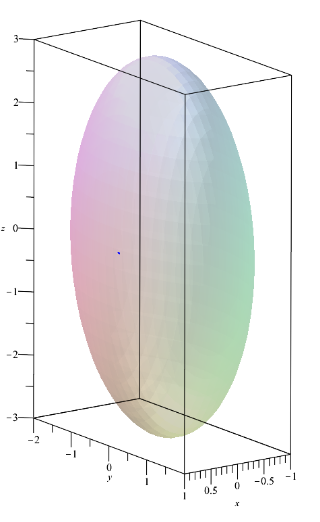
\includegraphics[width=0.3\textwidth]{ellipsoid1.png}
  \caption{egg\\Notes: the traces (like slices of the figure) are ellipses.}
  \label{fig:ellipsoid1}
\end{wrapfigure}
\underline{suppose $x=0$ ($zy$ plane):}
\begin{align*}
  \frac{0^2}{1}+\frac{y^2}{4}+\frac{z^2}{9}=1\\
  \frac{y^2}{4}+\frac{z^2}{9}=1
\end{align*}
\begin{flushleft}
  \underline{let $y=0$ ($xz$ plane):}
\end{flushleft}
\begin{align*}
  \frac{x^2}{1}+\frac{z^2}{9}=1
\end{align*}
\begin{flushleft}
  \underline{let $z=0$ ($xy$ plane):}
\end{flushleft}
\begin{align*}
  \frac{x^2}{1}+\frac{y^2}{4}=1
\end{align*}
\newpage
\begin{flushleft}
  \underline{let $y=1$}
\end{flushleft}
\begin{align*}
  \frac{x^2}{1}+\frac{1}{4}+\frac{z^2}{9}=1\\
  \frac{x^2}{1}+\frac{z^2}{9}=\frac{3}{4}\\
  \frac{x^2}{\frac{3}{4}}+\frac{z^2}{\frac{27}{4}}=1
\end{align*}

\subsection{Cones}

\begin{align*}
  &\frac{x^2}{16}+\frac{y^2}{81}=\frac{z^2}{256}\\
  \Rightarrow\quad&\frac{x^2}{16}+\frac{y^2}{81}-\frac{z^2}{256}=0\quad\surd
\end{align*}
\begin{figure}[H]
  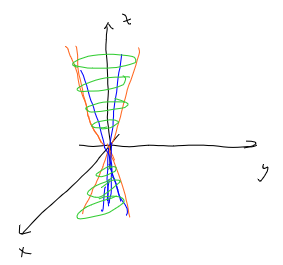
\includegraphics[width=0.4\textwidth, center]{cone1.png}
  %\caption{}
  \label{fig:cone1}
\end{figure}
\begin{flushleft}
  \underline{let $x=0$:}
  \begin{align*}
    \frac{y^2}{81}&=\frac{z^2}{256}\\
    \frac{y}{9}&=\pm\frac{z}{16}\\
    z&=\pm\frac{16}{9}y\\
    z&=\frac{-16}{9}y
  \end{align*}
  \underline{$z=c$}
  \begin{align*}
    \frac{x^2}{16}+\frac{y^2}{81}=\frac{c^2}{256}
  \end{align*}
  \underline{$y=0$}
  \begin{align*}
    \frac{x^2}{16}=\frac{z^2}{256}\quad\Rightarrow\quad z=\pm\frac{16}{4}x
  \end{align*}
\end{flushleft}

\subsection{Equations}
\begin{itemize}
  \item \textbf{Elliptic Paraboloid:}
  \[
  %\quad\qquad\qquad\qquad\qquad\qquad\qquad\qquad\qquad\frac{x^2}{a^2}+\frac{y^2}{b^2}=\frac{z}{c}
  \frac{x^2}{a^2}+\frac{y^2}{b^2}=\frac{z}{c}
  \]
  \item \textbf{Circular Paraboloid:}
  \[
  %\quad\qquad\qquad\qquad\qquad\qquad\qquad\qquad\qquad\frac{x^2}{a^2}+\frac{y^2}{a^2}=\frac{z}{c}
  \frac{x^2}{a^2}+\frac{y^2}{b^2}=\frac{z}{c}
  \]
  \item \textbf{Elliptic Cone:}
  \[
  \frac{x^2}{a^2}+\frac{y^2}{b^2}=\frac{z^2}{c^2}
  \]
\end{itemize}

\section{Hyperboloids}

\subsection{1 Sheet Elliptical Hyperboloid}
\begin{align*}
  \frac{x^2}{16}+\frac{y^2}{81}-\frac{z^2}{256}=1
\end{align*}
\begin{wrapfigure}{r}{0.35\textwidth}
  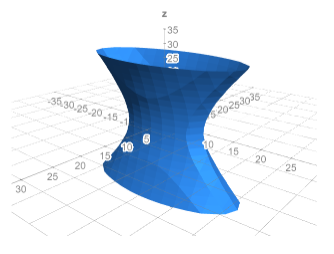
\includegraphics[width=0.5\textwidth]{hyperboloid1.png}
  \caption{``elliptical hyperboloid'' \& 1 sheet}
  \label{fig:hypberola1}
\end{wrapfigure}
\begin{flushleft}
  \underline{traces:}
\end{flushleft}
\begin{align*}
  &z=0\qquad\qquad\qquad\frac{x^2}{16}+\frac{y^2}{81}=1
\end{align*}
\hspace{5.85cm}(ellipse)
\begin{align*}
  &y=0\qquad\qquad\qquad\frac{x^2}{16}-\frac{z^2}{256}=1
\end{align*}
\hspace{5.85cm}(hyperbola)
\newpage
\begin{align*}
  &x=0\qquad\qquad\qquad\frac{y^2}{81}-\frac{z^2}{256}=1
\end{align*}
\hspace{5.75cm}(hyperbola)
\begin{flushleft}
  \begin{align*}
    \qquad z=16\quad\qquad\qquad&\frac{x^2}{16}+\frac{y^2}{81}-1=1\\
    &\frac{x^2}{16}+\frac{y^2}{81}=2\\
    &\frac{x^2}{32}+\frac{y^2}{162}=1
  \end{align*}
  \hspace{5.75cm}(hyperbola)
\end{flushleft}

What if we put the minus sign on the $y$ term?

\begin{align*}
  \frac{x^2}{16}-\frac{y^2}{81}+\frac{z^2}{256}=1
\end{align*}
\begin{wrapfigure}{r}{0.35\textwidth}
  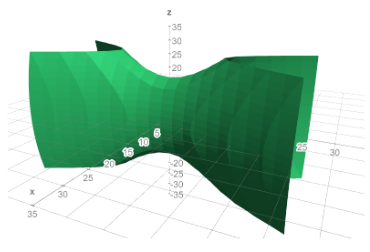
\includegraphics[width=0.5\textwidth]{hyperboloid2.png}
  %\caption{"elliptical hyperboloid" \& 1 sheet}
  \label{fig:hyperbola2}
\end{wrapfigure}
\begin{align*}
  &z=0\qquad\qquad\qquad\frac{x^2}{16}-\frac{y^2}{81}=1\\
  &y=0\qquad\qquad\qquad\frac{x^2}{16}-\frac{z^2}{256}=1\\
  &x=0\qquad\qquad\qquad\frac{z^2}{256}-\frac{y^2}{81}=1
\end{align*}

\newpage
\subsubsection{2 Sheet Elliptical Hyperboloid}

\begin{align*}
  \frac{x^2}{16}-\frac{y^2}{81}-\frac{z^2}{256}=1
\end{align*}
\begin{figure}[H]
    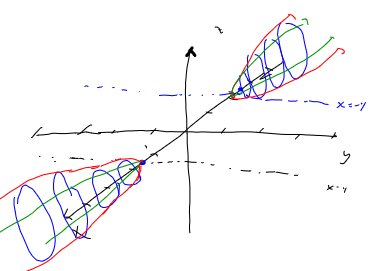
\includegraphics[width=0.4\textwidth, center]{hyperboloid3.png}
  \caption{2 sheets because there's 2 ``sheets'' between them.}
  \label{fig:hyperbola3}
\end{figure}
\begin{flushleft}
  \underline{let $x=0$:}
  \begin{align*}
    &\frac{y^2}{81}-\frac{z^2}{256}=1
  \end{align*}
  No solutions.
  \begin{align*}
    &\frac{y^2}{81}-\frac{z^2}{256}=1-\frac{x^2}{16}
  \end{align*}
  No solutions when $x>4$.

  \underline{let $y=0$:}
  \begin{align*}
    &\frac{x^2}{16}-\frac{z^2}{256}=1
  \end{align*}
  \underline{let $z=0$:}
  \begin{align*}
    \frac{x^2}{16}-\frac{y^2}{81}=1
  \end{align*}
\end{flushleft}

\subsection{Equations}
\begin{itemize}
  \item \textbf{1 Sheet Hyperboloid:}
  \[
  \quad\qquad\qquad\qquad\qquad\qquad\qquad\qquad\qquad\frac{x^2}{a^2}+\frac{y^2}{b^2}-\frac{z^2}{c^2}=1
  \]
  \item \textbf{2 Sheet Hyperboloid:}
  \[
  \quad\qquad\qquad\qquad\qquad\qquad\qquad\qquad\qquad\frac{z^2}{c^2}-\frac{x^2}{a^2}-\frac{y^2}{a^2}=1
  \]
  \item \textbf{Hyperbolic Paraboloid:}
  \[
  \frac{y^2}{b^2}-\frac{x^2}{a^2}=\frac{z}{c},\qquad c>0
  \]
\end{itemize}
\begin{figure}[H]
  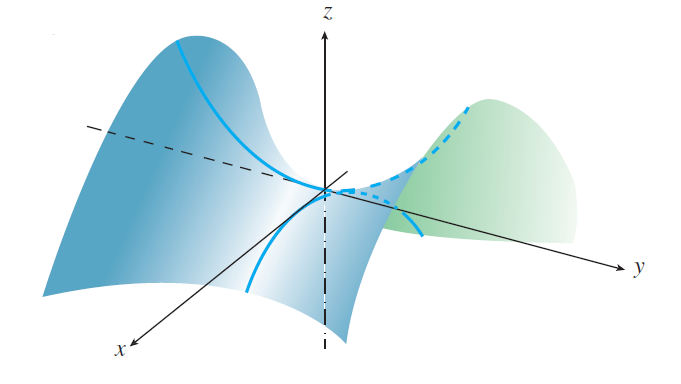
\includegraphics[width=0.4\textwidth, center]{hyperboloid4.png}
  \caption{A hyperbolic paraboloid.}
  \label{fig:hyperbola4}
\end{figure}


\end{document}
